\documentclass[11pt]{article}
\usepackage{url}
\usepackage{cite}
\usepackage{amsmath}
\usepackage{amsthm}
\usepackage{graphicx}
\graphicspath{{../../}}

\newtheorem{definition}{Definition}
\newtheorem{theorem}{Theorem}
\newtheorem{notation}{Notation}

\begin{document}

\title{Querying the Semantic Web with Natural Language}
\author{Ernest Kirstein}
\maketitle

\tableofcontents

\section{A Brief Introduction to the Semantic Web}
The semantic web (as invisioned by Tim Berners-Lee et al.) is an extention of
the internet which provides more structure to the vast chaos of data on the
net. The goal has always been for the semantic web to become
a means for AI agents to share information and reasoning \cite{semantic}.
The world wide web has it's foundation in HTML/CSS/JS documents and HTTP requests.
Similarly, the semantic web is rooted in RDF/OWL documents and SPARQL queries.

RDF documents are XML pages which
describe object types (classes), and instances of those types. 
They can also document relations between objects hierarchically or compositionally. 
RDF documents are quite expressive, in and of themselves. 

Then there are OWL ontologies which are RDF documents for describing relations
between RDF entities\cite{owl}. OWL is more technically specified in such a
way that it allows for further automated reasoning
over RDF data stores. RDF may make the semantic web expressive, but OWL
allows it to be intellegent.

To unlock the power behind the semantic web, there needs to be a way for people
to interface with it and ask questions about stored (or reasoned) information. 
One of the main interfaces is called SPARQL. 
SPARQL is a query language that is used to ask questions about semantic
data \cite{sparql}. The main benefit to this type of interface is that it allows users to ask
complex, exact questions. The main drawback is that, being a formal query language,
SPARQL has a steep learning curve and is only accessible to expert users.

The system I propose in this work attempts to make the semantic web more accessible
by allowing users to ask questions in natural language. That is, plain English.
The actuall implementation of this tool handels only a small range of questions,
but it does demonstrate promissing possibilities.

\section{Converting Natural Language Questions into \\SPARQL Queries}
Since SPARQL is already a well-worn tool for navigating the semantic
web, it make sence to leverage it. This system we have built recieves natural language
questions such as, ``What author has writen both high fantasy and science fiction?"
Then the system produces a SPARQL query which asks the same question. 
The end goal is to allow general users to achieve the same level of sophistication
as expert users using English rather than SPARQL.

Work by Kaufmann and Bernstein \cite{usability} indicates
that users have a “clear preference” for even limited natural language interfaces
when compared to keyword or query language interfaces.
Other recent works \cite{mapping, freya, galitsky}
have shown that simple natural language questions can be translated based
on known sentence structure using (among other things) NER, named-entity recognition.

These systems are limited - they generally only handle simple, direct questions.
A recent publication by Sharef et al. \cite{issues} outlines obstacles in developing full
natural language interfaces for the semantic web. That paper notes a particular
difficulty with parsing what we call `multifaceted' questions - questions with multiple
variables, constraints, or operations. This is the precise gap which this work
attempts to bridge.

The foundations of both compiler design and natural language processing
have significant overlap \cite{chomsky, reghizzi}.
However, in practice, there has not been
much synergy between the two disciplines \cite{aho, anatomy, reghizzi}.
I believe cooperation between these astranged fields is necessary to move forward
in either.

Our approach was be to build a ``natural language compiler" of sorts.
That is, to approach the problem of converting natural language questions into
SPARQL queries just as one might convert Java source code into byte code.
The problems are, or course, an order of magnitude appart in complexity.
So our only aim was only to parse a limited range of natural language questions.
But in that range of questions, we intend to show that multifacited questions
can be handeled on a limited basis.

\subsection{Named Entity Recognition}
Different types of named objects are recognized as part of the parsing process.
Since the names are matched durring parsing, the NER is greatly improved by context.
Still, this matching requires a bit of preprocessing.

Statistical character models are constructed from the output of queries for all 
objects of a certain type in the target RDF database. 
These models are used to recognize arbitrary tokens (or combinations of 
tokens) within the parser's grammar. 

These models allow for probablistic recognition of the input strings in 
$O(1)$ time (at least, in relation to the number of objects in the RDF
database). They recognize variations on the names (typos, variations, etc.)
within some user-defined bound. 

\subsection{Parsing}

TODO: Insert General Introduction to Top-Down Parsing 

This system uses a custom parser which has been implemented especially for
this project. One of the contributions of this work is the unique implemtation
of this parser. The parser automatically handles left recursion and a few other
hiccups which usually give top-down parsers trouble. However, the parse trees
(which the parser outputs) retain the original structure of the initial grammar.
This is accomplished by reversing the transformation required to remove left
recursion (etc.).

\begin{figure}[h!]
    \centering
    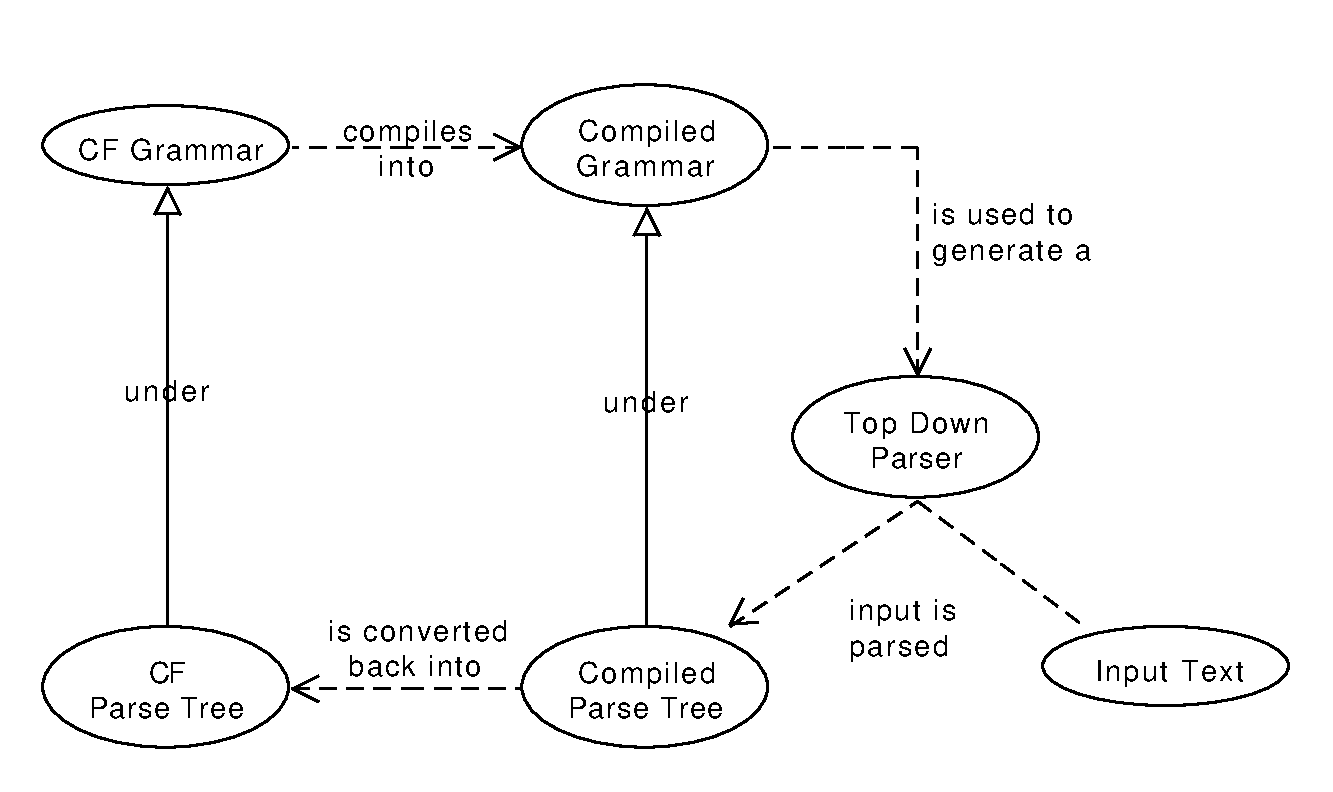
\includegraphics[width=0.9\textwidth,natwidth=1,natheight=1]{umlet/high_level.pdf}
    \caption{A high level overview of the parsing process.}
    \label{fig:high_level_parse}
\end{figure}

The grammar generated to handel the natural language questions
is composed of rules which handle each type of question.
The `type' of question is vague: it is largely a matter of design preference.
The broader the scope of a `type', the harder it will be to develop a grammar
which recognizes that question. But the narrower the types, the more types
will need to be implemented to cover the same range of questions.

\begin{figure}[h!]
    \centering
    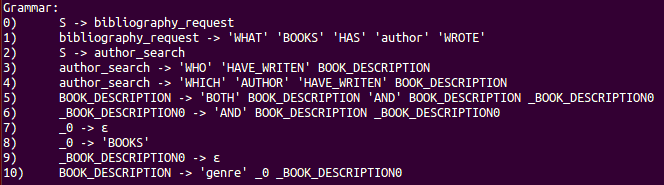
\includegraphics[width=1\textwidth,natwidth=1,natheight=1]{imgs/demo/grammar.png}
    \caption{Grammar}
    \label{fig:grammar}
\end{figure}

Grammar rules are defined for each question, then compiled into a single
unified grammar (see figure \ref{fig:grammar}) with left recursion and other such 
nuisances automatically `compiled' into the grammar. 
Again, that is to be discussed in a later section.

\begin{figure}[h!]
    \centering
    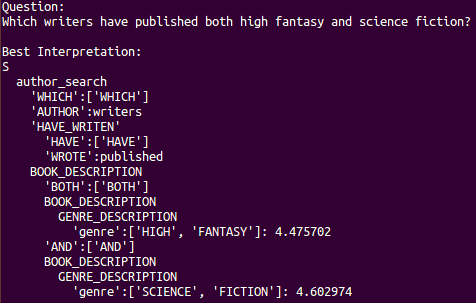
\includegraphics[scale=1.0,natwidth=1,natheight=1]{imgs/demo/parse.png}
    \caption{Input and Parse Tree}
    \label{fig:parse}
\end{figure}

Given a natural language question, the parser then produces a number of
parse trees and selects the "best" (most probable) interpretation. That
interpretation 

\subsection{Resolution}
After parsing, specific instances of named entities need to be 'resolved' to
corresponding RDF entities. Natural language names (like "John Smith") are mapped
to RDF URIs (like "http://sbc.net/smith394")
in a semi-automated process. This boils down to searching a
database of names with a good fuzzy string matching algorithm and falling
back on the user to select the appropriate name when there is no obvious best 
match.

A lot of work went into selecting the best fuzzy matching algorith for
natural language names. Thought Levenshtein's `edit distance` metric
is a good 

\subsection{Compilation}
Compiling SPARQL queries from the resolved parse trees is the last step.
For each type of question, there will be a separate unit which 
generates SPARQL queries. There might be a more elegant way to handle this
problem, but this seems like an extensible (if tedious to implement) solution.
Generation is often just a matter of fitting RDF URIs into hard-coded templates.

\begin{figure}[h!]
    \centering
    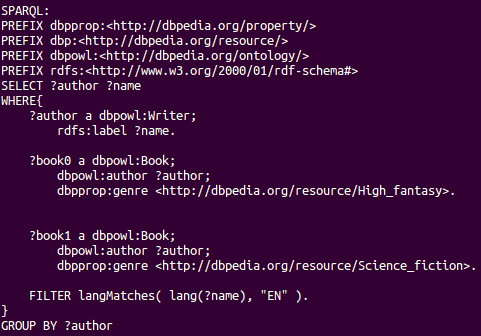
\includegraphics[width=1\textwidth,natwidth=1,natheight=1]{imgs/demo/sparql.png}
    \caption{SPARQL Output}
    \label{fig:sparql}
\end{figure}

\section{Software Architecture}

This architecture is aimed at handling complex questions in a narrow domain.
It does more than named entity recognition - it actually considers
the full syntax of the language and processes natural language questions
much like a compiler might process source code. It uses
top-down parsing to generate a parse tree for the input question then
compiles SPARQL queries from that parse tree.
This section will explain the design of the system at the highest level.

\begin{figure}[h!]
    \centering
    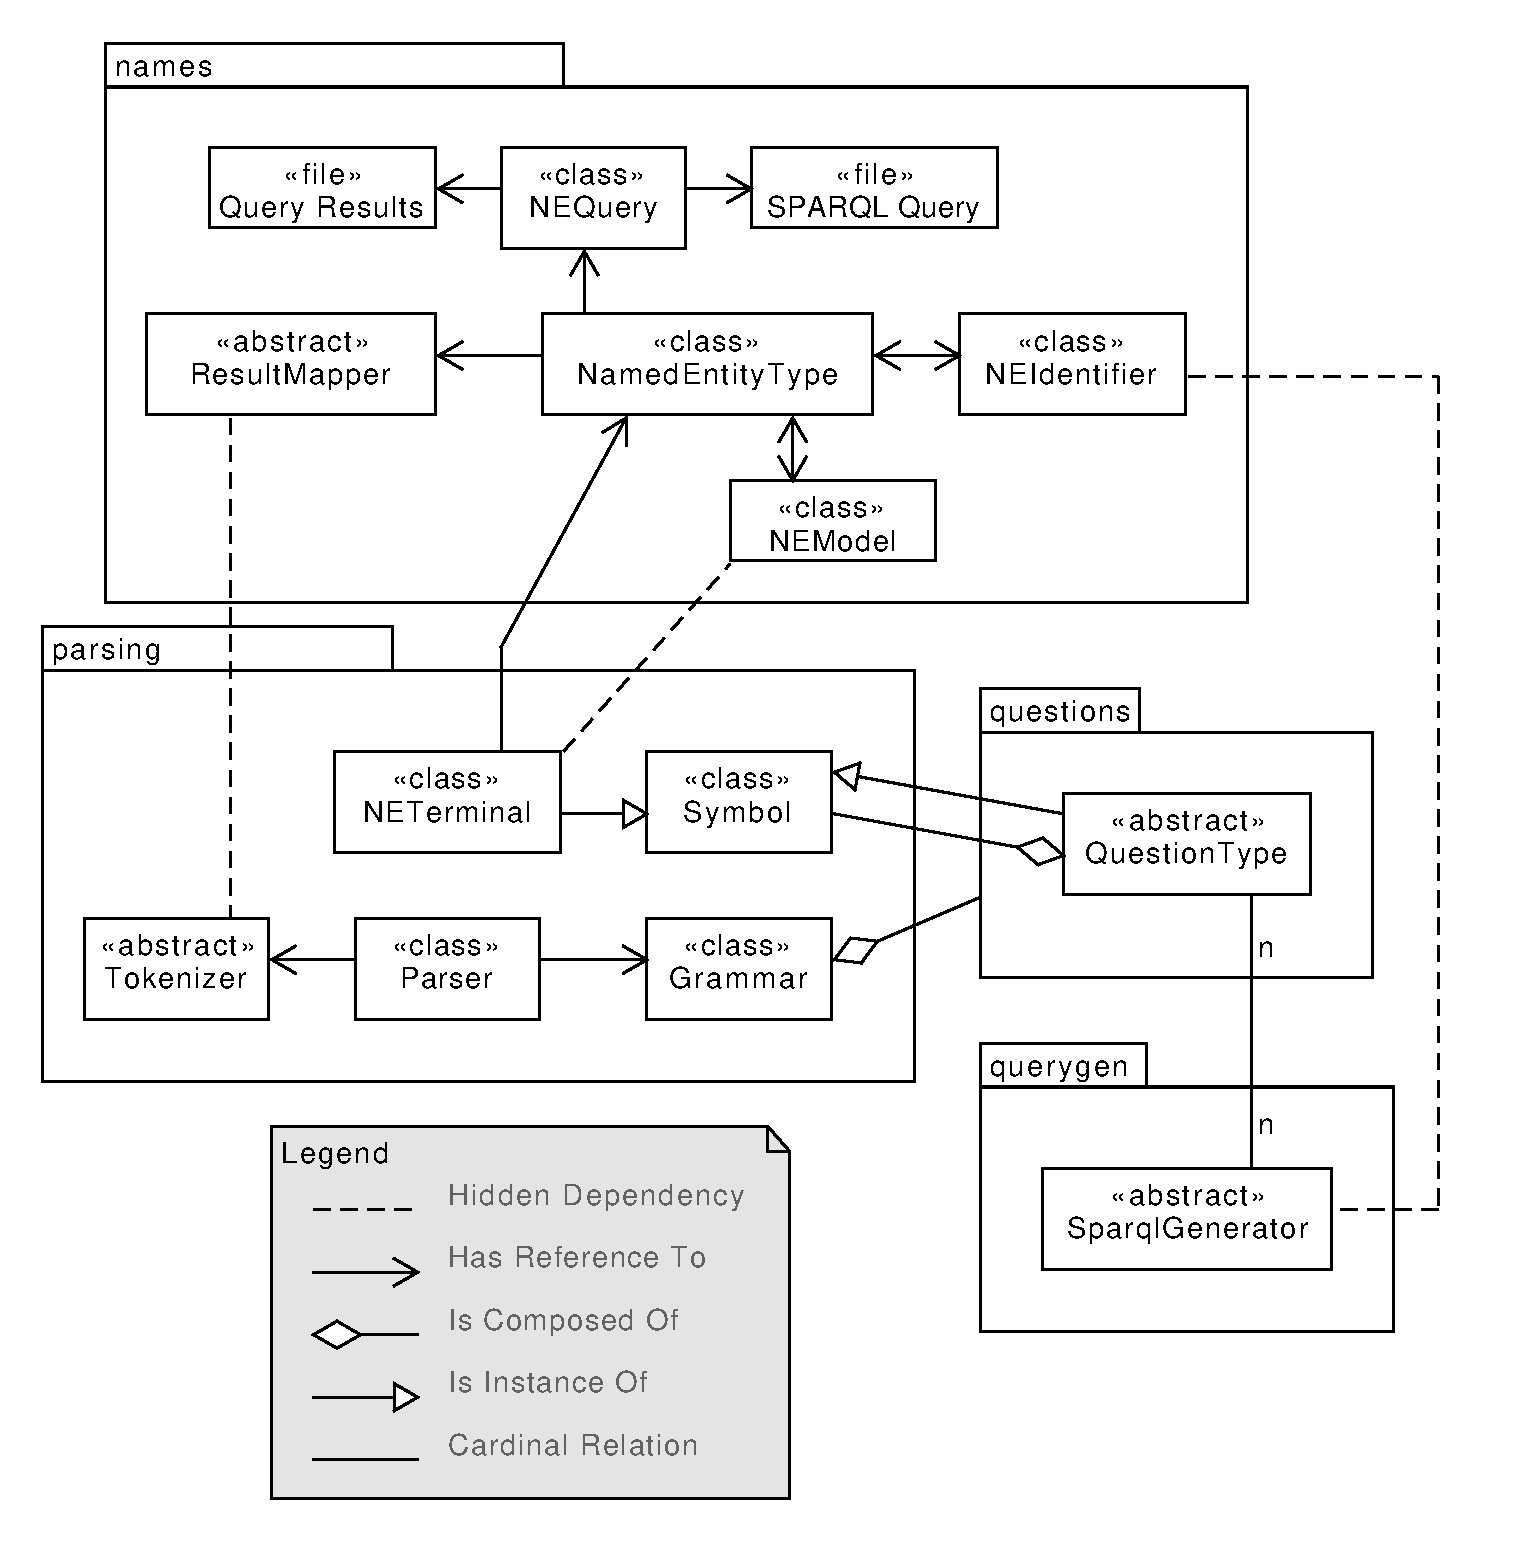
\includegraphics[width=0.9\textwidth,natwidth=1,natheight=1]{umlet/architecture.pdf}
    \caption{Architecture}
    \label{fig:arch}
\end{figure}


One of the goals of this project was to develop a
highly extensible architecture. There wasn't enough time to cover the
breadth of questions one would hope for in a mature product - such being
the nature of research. But I felt it was important to create a practical
working system that could handle a wide range of questions if more
time was dedicated towards that end.

To make the system extensible, it was important to decouple the various
components as much as possible. Still - language processing is a naturally
interdependent process with many overlapping concerns. For instance,
parsing seems to be an independent problem from named entity recognition (NER),
but to achieve better parsing results it was necessary to integrate NER into the
parser so that semantic context could inform the NER. 

\begin{figure}[h!]
    \centering
    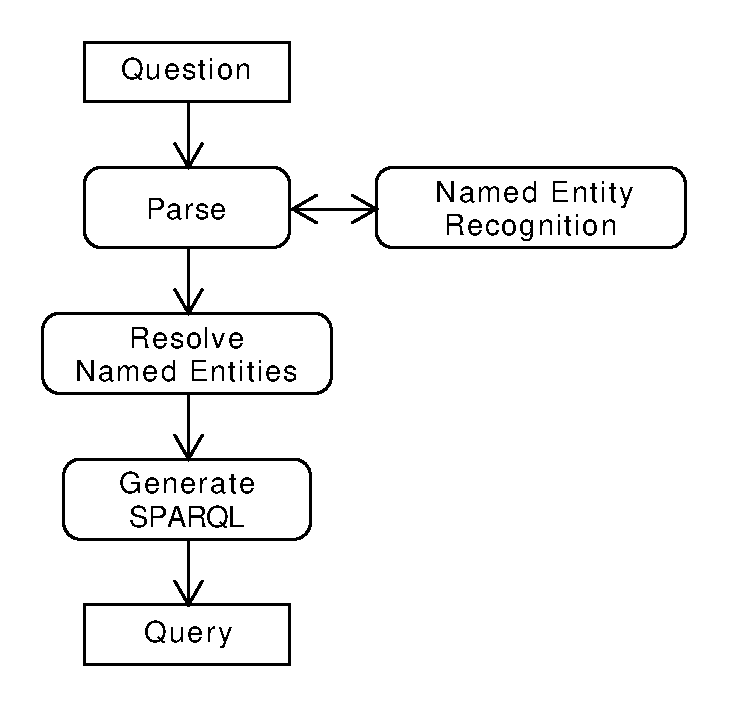
\includegraphics[width=0.5\textwidth,natwidth=1,natheight=1]{umlet/usage.pdf}
    \caption{Process}
    \label{fig:process}
\end{figure}

Another design concern was the accessability of the SPARQL endpoint.
It would be ideal if the endpoint was always accessable, would accept an unlimited
number of queries, and would always respond quickly. But in practice, none of
those ideals are true. As such, the results of certain queries
(necessary for developing NER models and URI resolution) are cached into local files.
The tradeoff is that data in the cache can stagnate. That problem is mitigated by 
simply flushing the cached results periodically.


\section{Resolving User Input Names to RDF Entities}

Matching natural language names to RDF entities is essential to evaluating
natural language questions over RDF databases. This poses several problems:
names can be misspelled (e.g. "Swartseneger" for the label "Schwarzenegger"), 
may be reordered (e.g. "John Smith" for the label "Smith, John"),
or the name may be abbreviated (e.g. "R.L. Stine" for the label "Robert Lawrence Stine").
That's not to meantion the small problem posed by people who have
changed their name entirely, sometimes multiple times
(e.g. "The artist formerly known as 'The artist formerly known as Prince'").
And despite all of these convolutions, a natural language system will need to
recognize and match these arbitrary instances with the often-sparse naming information
present in RDF data.

My approach to this problem was to find a string distance function which was
robust to these changes and use that to simply
find the best match name in $O(n)$ time. Since the names are narrowed down by
context (using the parser), this was an acceptable solution: we don't need to iterate
over every single label in the RDF set, just those which belong to the particular
type of object the user is asking about.

There are a surplus of string comparison functions to choose from \cite{comparison}.
For my particular application, I have used a varation on the {\em Jaccard index}.
It is robust to mispellings and reorderings, with the added benefit of being quite efficient.
The Jaccard index is used in datamining for efficiently comparining long documents,
but it is comparable to other more complex methods of name comparison \cite{comparison} and 
anecdotal evidence suggests it will work well here.

Another problem is resolving multiple close names (or even exactly the same name) to a single entity.
I took a simplistic approach (just asking the user) but I will also discuss other more
sophisticated possibilities for further research. 

\subsection{Name Standardization and Enumeration}
Before jumping into the specifics of the name comparison algorithm, there are a few trivialities
to deal with. Names with abbreviations, punctuation, and names with multiple parts can all
trip up comparison algorithms.

One standardization method I used was to remove punctuation and change all letters to upper case.
There may be a few edge cases where "John O'neal" isn't the same as "John Oneal",
but the mistake is acceptable the majority of the time. And such names are so close that they would
trigger the system to prompt the user for confirmation anyways.

Names with multiple parts, like "John Jacob Jingleheimer Schmidt", need to be matched by
partial variation like "Schmidt", "Mr. Schmidt", and "John Schmidt". 
Using a sufficieintly robust string comparison function, these variations will often 
still match the full, multi-part name better than other multi-part names.
But that's a dubious assumption to rely upon - it's best to tokenize the name and
include the different partial variations as other names linked with the entity.
As part of my own system, I simply included the first and last names as variations on
the name, excluding the middle name(s).

\subsection{Jaccard Index}
The Jaccard index is a measure of how similar two sets are to each other.
This is useful in a whole host of applications \cite{general}, as you might imagine. 
In this application, using the Jaccard index on fragments of strings yields a very
robust string comparrison function.

Let $A$ and $B$ be sets or multisets, then the Jaccard index $J(A,B)$ is defined \cite{mining, comparison}:
\begin{align*}
    J(A, B) = \frac{\left| A \cap B \right|}{\left| A \cup B \right|}
\end{align*}
Or if both sets are empty, $J(A,B) = 1$.
For comparing strings, the sets might be of characters (e.g. 'HELLO' $\mapsto \{E, H, L, O\}$), 
of tokens (e.g. 'JOHN H SMITH' $\mapsto \{\text{'JOHN'}, \text{'H'}, \text{'SMITH'}\}$),
or in this case, {\em n-grams}.

These n-grams (also known as 'k-grams' or 'shingles' \cite{mining}) are all unbroken substrings of 
length $n$ of a given string. So the 3-grams of the string 'anabasis' are 
$\{\text{'ana'}, \text{'nab'}, \text{'aba'}, \text{'bas'}, \text{'asi'}, \text{'sis'}\}$. 

In this application, n-grams were constructed to include imaginary pre and post string characters
(represented here as '\^{}' and '\$' respectively). So, for instance, the 3-grams of 'cat' are then
$\{\text{'\^{}\^{}c'}, \text{'\^{}ca'}, \text{'cat'}, \text{'at\$'}, \text{'t\$\$'}\}$. This gives
significance to the begining and end of a string when using the Jaccard index with the n-grams.

For a distance function, one can use:
\[d(s_1,s_2) = 1-J(ngrams(s_1),ngrams(s_2))\]
This doesn't produce a true metric space for the strings
(since two different strings can have exactly the same n-grams), but it does satisfy
the triangle inequality \cite{general} and is always non-negative. As such, one could
concievably construct an M-tree \cite{mtree} to improve lookup speed. That hasn't been necessary
in this research, but then again, this domain might be smaller than one might experience in
practice.

\subsubsection{Comparison with Levenshtein (Edit) Distance}
Levenshtein distance (also known as 'edit distance') is a more common fuzzy string comparison algorithm
than the Jaccard index. 
Its ubiquity might be due to a simple happenstance: the algorithm for calculating edit distance is
a favorite example in algorithm design courses for demonstrating dynamic programming.
But it's popularity is by no means a guarantee that it is the best choice, as I'll demonstrate.

Levenshtein distance is define as \cite{levenshtein} the minimum number of 'edits' 
(additions, deletions, or swaps) that must occur before one string matches another.
But these are only single-character edits, and so the algorithm doesn't handle large displacements
of parts of the name with any sort of grace.
This is best demonstrated by example; see figure \ref{fig:lev_comp}.

\begin{figure}[h!]
    \centering
    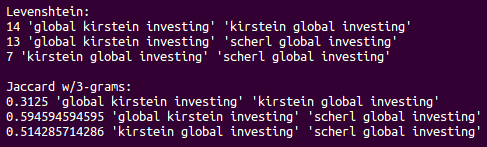
\includegraphics[width=0.9\textwidth,natwidth=1,natheight=1]{imgs/levenshtein_comp.png}
    \caption{Bad Levenstein Name Matching}
    \label{fig:lev_comp}
\end{figure}

Using levenshtein distance to match 'closest' strings, word 
inversions would be considered bulk deletions and insertions. 
The Jaccard index handels this better because inverting whole words 
still preserves the ngrams within those words even if it breaks
the joining ngrams between the words.

Admitedly, the Jaccard index is less forgiving of small typos. 
A single character edit breaks $n$ n-grams. So, for short single
word names, levenshtein distance is probably the prefered metric.

\subsubsection{Information Content Sensitive Jaccard Index}
The Jaccard index by itself is a fairly good way to compare names.
But it would be better if the algorithm also noticed things like
how 'unusual' certain name patterns were. 
"Tom Smith" might be closer to "John Smith" than "Tom" based purely
on their Jaccard index, but any reasonable person would pick
"Tom Smith" and "Tom" to be the closer names because "Smith" is
such a common surname.

In more technical terms, the part of the string "Smith"
should recieve less 'weight' in the comparison function because
it conveys less information. 

Consider the more general form of the Jaccard index \cite{general}:
\begin{align*}
J(\vec{x},\vec{y}) = 
\frac{\sum_i \min(x_i, y_i)}{\sum_i \max(x_i, y_i)}
\end{align*}
Where $\vec{x}$ and $\vec{y}$ are large dimensional vectors rather 
than sets. To help relate it back to the origional form, 
imagine that $\vec{x}$ and $\vec{y}$ are lists
of counts of all the possible things that could be in the two sets
(or multisets) $A$ and $B$.
\begin{align*}
x_i = count(e_i; A)\\
e_i \in \{A \cup B \}
\end{align*}

Now if we want to consider the amount of information each little
portion of the string contains, we can calculate it
using the equation layed down by Shannon \cite{shannon}.
Namely, that the self information of an event is the log of the
inverse of the probability that event occuring. In this case,
the 'event' is the occurence of a certain n-gram in the string.

\begin{align*}
I(e_i) &= \log\left(\frac{1}{P(e_i)}\right)\\
&= -\log(P(e_i))
\end{align*}

To determine this probability, we can look at the frequency
of the n-gram in a large sample set of names.
We need to index those names anyways, as part of the named entity
recognition proces. With a large set, we can get pretty close to a true 
approximation of the probability of an n-gram occuring in 
a general population of those names:

\begin{align*}
P(e_i) \approx \frac{count(e_i; N)+1}{|N|+2}
\end{align*}

Where $N$ is the multiset containing the union of all the n-grams of
all the names. 
Then, we can weight the vectors $x$ and $y$ such that we have
an information sensitive comparision function: $\hat{J}(x,y)$:

\begin{align*}
\hat{J}(\vec{x},\vec{y}) &= \frac{
    \sum_i \min(x_iI(e_i), y_iI(e_i))
}{
    \sum_i \max(x_iI(e_i), y_iI(e_i))
}\\
&= J\left(\vec{x} \cdot \vec{I}, \vec{y} \cdot \vec{I} \right)\\
\vec{I} &= \left< I(e_1), I(e_2), ... I(e_n) \right>
\end{align*}

\begin{figure}[h!]
    \centering
    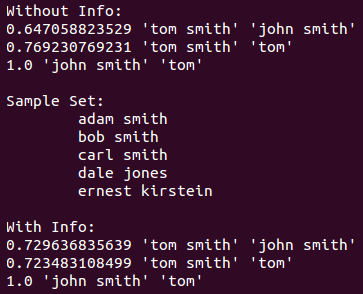
\includegraphics[width=0.6\textwidth,natwidth=1,natheight=1]{imgs/info_comp.png}
    \caption{Information Sensitive Name Matching}
    \label{fig:lev_comp}
\end{figure}

The above example shows this comparison in action. In the top comparision,
without considering information content, the closest pair of names is
"tom smith" and "john smith". But after indexing the sample names, we
can calculate comparisons that do consider the information content. Then
we can see that the closer names are "tom smith" and "tom".

\subsection{Ambiguity}
What should the system do when the user inputs a name which is close
to the names of several entities by the chosen name comparision
function? The easiest solution would be to simply ask the user which
of the possible entities they meant. But this isn't always a great
solution; what if you're asking about a cornicopia of names?
Sure, it might be out of scope for this particular system to
resolve questions such as "Which of the actors in 'my\_data\_file.txt'
have been in movies together?" But that's certainly within the
realm of possibilities for some future work.

One approach to this problem would be to create a separate
system for distinguishing the "right" name from a small(er) selection
of possible candidates. The aformentioned Jaccard index (or similar
distance metric) might be used to narrow down the problem space
to something managable, then a much more sophisticated (yet slower)
system could choose the right name from the smaller set.

Since there are a number of string comparison algorithms, one could
(if time permited) implement several of them and use a combigned
metric to evaluate the names for fitness. For example,
a feed-forward neural net could be trained to recognize the 'right'
name based on a number of factors:
\begin{itemize}
\item String comparison functions (Jaccard, Levenshtein, etc.)
\item The self-information \cite{shannon} of the input and potential match names
\item The closeness of other potential match names
\item The prevelance of the potential match entity in the RDF data
\item The frequency of queries involving the potential match entity
\item Etc.
\end{itemize}

\section{Top-Down Parsing}
Historically, top-down parsers were been coded manually or else generated from 
a context free grammar specification. \cite{lewis, formal_langs} 
Coding a RDP manually is tedious, error prone, and difficult to maintain.
Programatically generating a top-down parser from a grammar
still isn't ideal - converting a context free grammar into
a top-down parsable form may not preserve the {\em strong equivalence} of the grammar.
And as a result, parse trees generated by that RDP will not be in the same form
as they might appear in the initial (non-RD-parsable) grammar, which is often a more 
natural representation of the desired language \cite{compiler}.

In this work, we hope to describe a useful adaptation to top-down parseing
which addresses these problems. Our system compiles a context free grammar 
specification into a top-down parseable grammar.
A parser is generated from the top-down parseable gramar,
and used to parse a input streams. 
The resulting parse trees are then transformed back into equivalent
parse trees under the original grammar. (Figure \ref{fig:high_level_parse})

\subsection{Introduction to Top-Down Parsing without Syntax Diagrams}
\label{rd_wo_sd}
Introductory material by Dr. Lewis \cite{lewis} describes a recursive-descent parser 
as a piece of software which takes a sentence and turns it into a parse tree by performing a 'depth-first' search. 
But a search of what? One might try to call it a search of the parse tree, but that's not exactly right.
The 'recursive descent' name comes from the way that a RDP traverses through a
syntax diagram of a context free grammar \cite{compiler}.

Recursive decent is just one form of top down parsing. The top-down parsing in this thesis
does not use sytax diagrams (in hindsight, this was a questionable design choice, 
but such is life). This section will describe how top-down parsing works without
using syntax diagrams.

Consider a context-free grammar with the following production rules:
\setcounter{equation}{0}
\begin{align}
S &\rightarrow a S\\
S &\rightarrow b S\\
S &\rightarrow \epsilon
\end{align}
And the following string which we will attempt to parse: "ab"

We know, right off the bat, that the start symbol $S$ will be the root of any parse tree created under this
grammar, by virtue of it being the start symbol. (Figure \ref{fig:rdp_0})

\begin{figure}[h!]
    \centering
    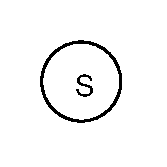
\includegraphics[natwidth=15,natheight=15]{umlet/rdp_0.pdf}
    \caption{Parse Tree 0}
    \label{fig:rdp_0}
\end{figure}

The next parse tree we should consider is the parse tree that is generated when we follow the first 
production rule. (Figure \ref{fig:rdp_1}) Notice that, in this instance, the parse tree does not conflict with
the string we are trying to parse - i.e. regardless of the production rules we follow the string that is
produced from any further production rules we follow will start with "a".

\begin{figure}[h!]
    \centering
    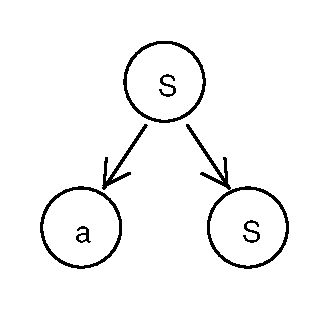
\includegraphics[width=0.4\textwidth,natwidth=30,natheight=30]{umlet/rdp_1.pdf}
    \caption{Parse Tree 1 - Valid}
    \label{fig:rdp_1}
\end{figure}

For the next parse tree, we will try to repeat are last action (following the first possible production rule).
(Figure \ref{fig:rdp_2}) This parse tree conflicts with the string we are trying to produce since any
string produced by further production rule applications will produce a string starting with "aa".
In this case, we go back to the previous parse tree and try a different production rule.

\begin{figure}[h!]
    \centering
    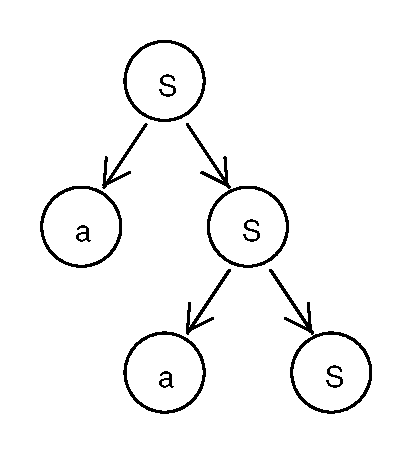
\includegraphics[width=0.4\textwidth,natwidth=30,natheight=30]{umlet/rdp_2.pdf}
    \caption{Parse Tree 2 - Invalid}
    \label{fig:rdp_2}
\end{figure}

In figure \ref{fig:rdp_3}, we've followed the second production rule
and our new parse tree fits with the input string, so we can continue our descent.

\begin{figure}[h!]
    \centering
    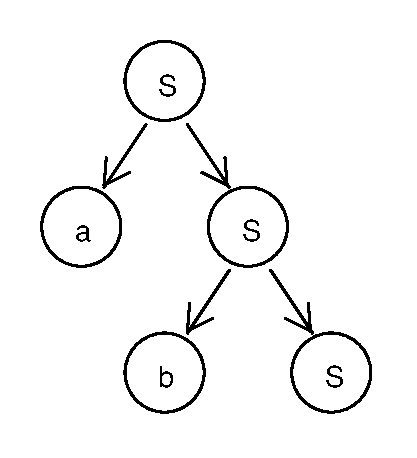
\includegraphics[width=0.4\textwidth,natwidth=30,natheight=30]{umlet/rdp_3.pdf}
    \caption{Parse Tree 3 - Valid}
    \label{fig:rdp_3}
\end{figure}

The next two parse trees (Figure \ref{fig:rdp_4_5}), created by applying the first and second production rules to
Parse Tree 3, are both invalid because they extend past the length of our input string.

\begin{figure}[h!]
    \centering
    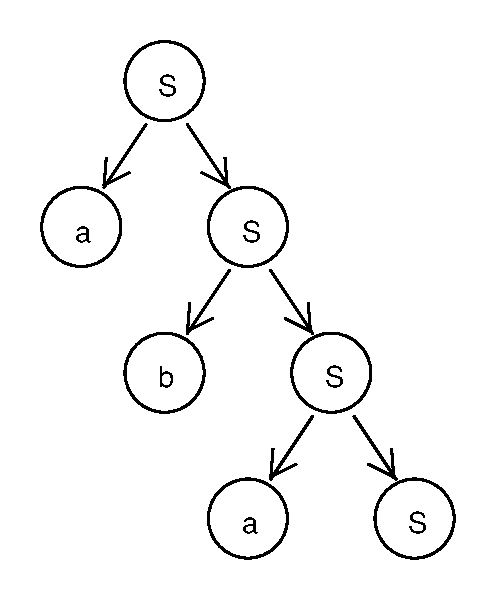
\includegraphics[width=0.4\textwidth,natwidth=30,natheight=30]{umlet/rdp_4.pdf}
    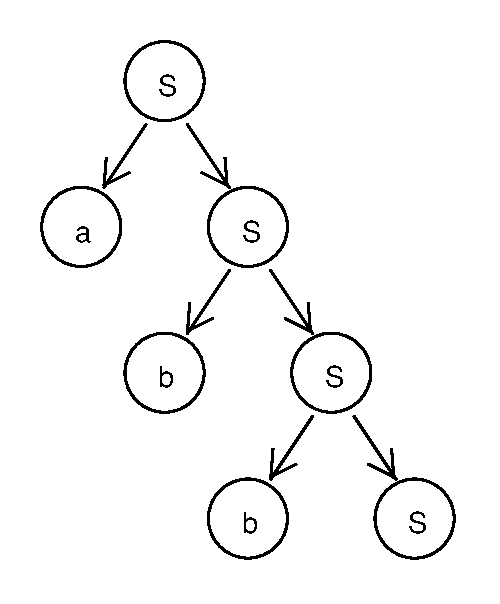
\includegraphics[width=0.4\textwidth,natwidth=30,natheight=30]{umlet/rdp_5.pdf}
    \caption{Parse Trees 4 and 5 - Both Invalid}
    \label{fig:rdp_4_5}
\end{figure}

In the last step, by applying the third production rule to Parse Tree 3, we have a parse tree which terminates and produces the
desired input string, "ab". (Figure \ref{fig:rdp_6})

\begin{figure}[h!]
    \centering
    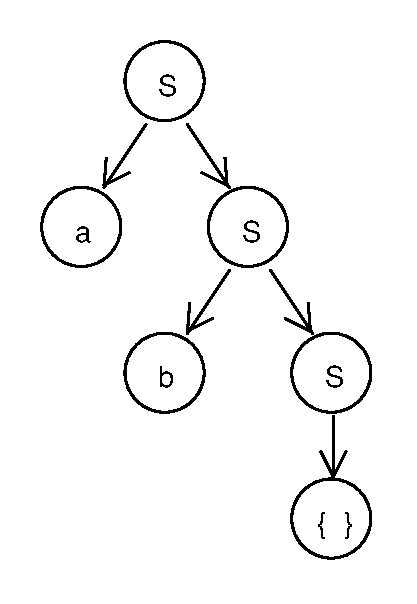
\includegraphics[width=0.4\textwidth,natwidth=30,natheight=30]{umlet/rdp_6.pdf}
    \caption{Parse Tree 6 - Complete}
    \label{fig:rdp_6}
\end{figure}

Finally, let's diagram our traversal through the possible parse trees (Figure \ref{fig:rdp_7}). Shown this way, one can notice
a pattern in our attempt to build the tree. The top-down parser performs a depth first search of the 
graph of possible parse trees, looking for a parse tree which fits the input string.
The child nodes from each PT (Parse Tree) node in the graph are PT nodes generated by
applying each of the production rules to the first (left, deepest) nonterminal symbol in that PT node.
The depth of each node in the PT tree corresponds with the number of production rules that have been applied.

\begin{figure}[h!]
    \centering
    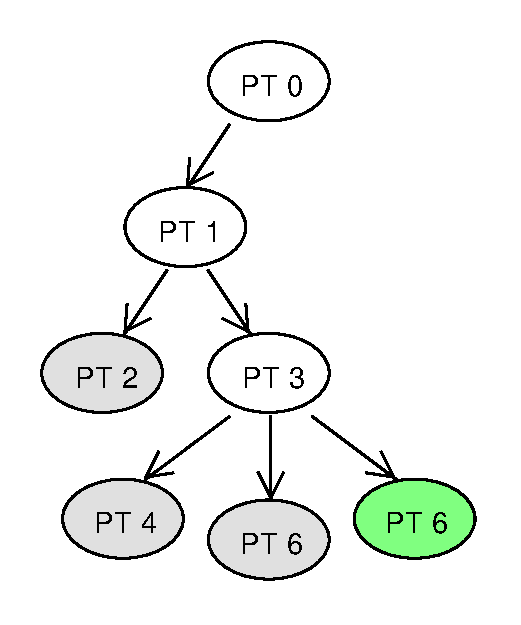
\includegraphics[width=0.4\textwidth,natwidth=30,natheight=30]{umlet/rdp_7.pdf}
    \caption{Parse Tree Search Progression}
    \label{fig:rdp_7}
\end{figure}

\clearpage

\subsection{Effect of Grammar Transformations on Parse Trees}
Left recursion is a problem for top-down parsers because it may cause them to
go into an infinite loop. Using the model described in section \ref{rd_wo_sd}:
when a PT node is reach where the first non-terminal symbol has a production rule with
left recursion, it's child node will have the same non-terminal symbol so it will produce
a child node with the same non-terinal symbol ad infinitum - and none of those children will
consume any terminals from the input stream so the parser will not proceed. 

So, removing left recursion from context free grammars is a necessary evil for top-down parsing.
It just takes two transformations to turn any context free grammar with left recursion
into a {\em weakly equivalent} grammar with only right recursion.
These two transformations are direct left recursion elimination, 
$DLRE(G; R_\alpha, R_\beta) \rightarrow G'$ and substitution, 
$Sub(G; r_\alpha, R_\beta) \rightarrow G'$, which is used to
remove indirect left recursion. \cite{aho, lewis}
These sections will describe how these transformations work on the grammar
and on their parse trees.

\subsubsection{Direct Left Recursion Elimination}
A left recursive grammar, $G$, has rules for some non-terminal $A$ of the form
$A \rightarrow A \alpha_i$ and $A \rightarrow \beta_j$, $i \in [1,m]$, $j \in [1,n]$.
Let $R_\alpha$ and $R_\beta$ represent the sets of those rules respectively where the notation
$R_\alpha(1)$ represents $A \rightarrow A \alpha_1$. 
Such a grammar represents a language which contains strings of the form
$\beta_y \alpha_{x_1} \alpha_{x_2} ... \alpha_{x_p}...\alpha_{x_{k-1}} \alpha_{x_k}$ where $y \in [1,m]$ and each $x_p \in [1,n]$.
However, to produce such a string, the alpha rules need to be followed in reverse order:
\[R_\alpha(x_k), R_\alpha(x_{k-1}), ... R_\alpha(x_{p}), ... R_\alpha(x_2), R_\alpha(x_1), R_\beta(y)\]

The transformation \cite{aho} $DLRE(G; R_\alpha, R_\beta) \rightarrow G'$ changes
each rule in $R_\alpha$ to the form $A' \rightarrow \alpha_i A'$, each rule
in $R_\beta$ to the form $A \rightarrow \beta_j A'$, and adds an additional rule
$R_\epsilon = A' \rightarrow \epsilon$. Consequently, the order of the followed production
rules in $G'$ results in alpha rules being followed in forward order:

\[R_\beta(y), R_\alpha(x_1), R_\alpha(x_2), ... R_\alpha(x_p), ... R_\alpha(x_{k-1}),R_\alpha(x_k), R_\epsilon \]


\begin{figure}[h!]
    \centering
    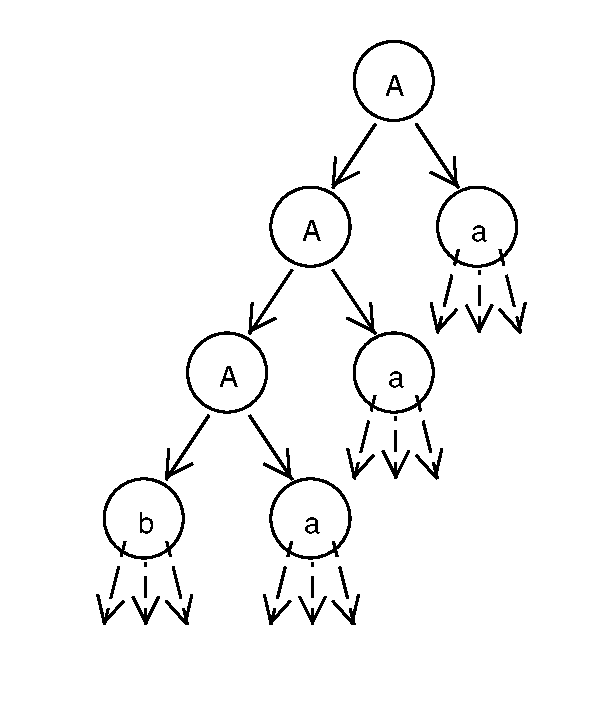
\includegraphics[width=0.4\textwidth,natwidth=1,natheight=1]{umlet/dlre_orig.pdf}
    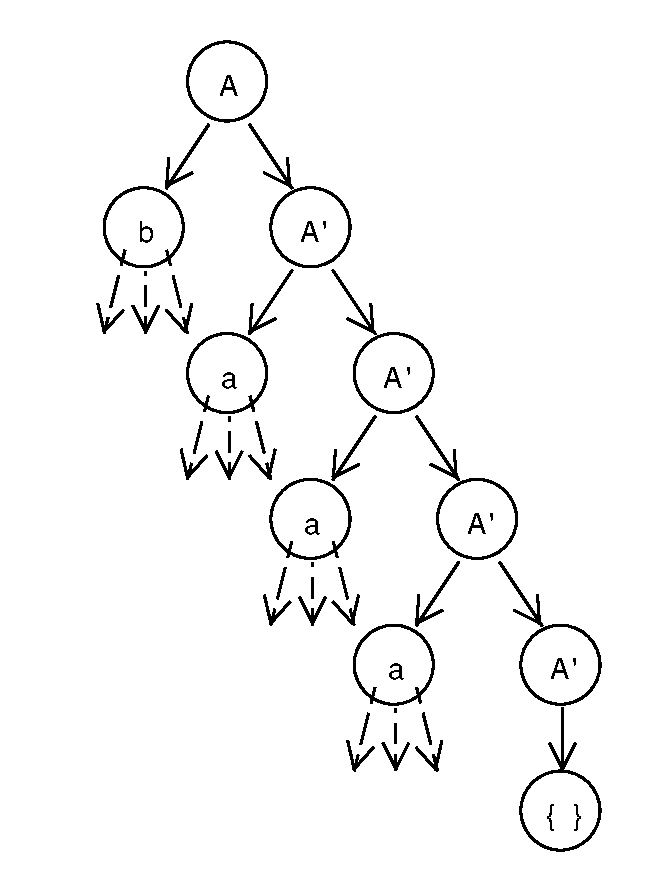
\includegraphics[width=0.4\textwidth,natwidth=1,natheight=1]{umlet/dlre_comp.pdf}
    \caption{Original and Transformed Parse Trees}
    \label{fig:dlre}
\end{figure}

The transformation effects the parse trees by flipping and reversing $A$ chains,
replacing lower $A$ nodes with $A'$ nodes, moving the $\beta$ up,
and adding an $A'$ node and $\epsilon$ node to the end of the chain. (Figure \ref{fig:dlre}) The inverse transformation
removes last $A'$ and $\epsilon$ nodes, moves the $\beta$ back down to the end of the chain, and changes the $A'$ nodes back into
$A$ nodes, then flips and reverses the $A$ chain. Note that the $\alpha$ and $\beta$ nodes are arbitrary strings, so in reality
they might be multiple nodes which might have any number of children.

More formally, for each $A$ node in the RD-parsable grammar, the inverse transformation $DLRE^{-1}(T'; A, A') \rightarrow T$
modifies chains of $A/A'$ nodes where the children of the $A$ node are $C_A$, of all but the last $A'_{x_p}$ node are $C_{A'_{x p}}$,
and the last $A'_\epsilon$ node has only the child $\epsilon$.
From the $DLRE$ transformation rules we know that the $C_A$ will be of the form $\beta_y A'_{x_1}$. 
We can also conclude from the $DLRE$ tranformation that each $C_{A'_{x p}}$ will be of the form $\alpha_p A'_{x_{p+1}}$
when $p < k$ and $A'_\epsilon$ when $p=k$. 

The inverse transformation first removes the $A'_\epsilon$ node. Then it changes each remaining $A'_{x_p}$ node into an $A_{x_p}$ node
with the same children. Next the $A_{x_p}$ are restructured such that each $C_{A_{x p}}$
is equal to $A_{x_{p-1}} \alpha_p$ where $1 < p$ and $\beta_y \alpha_k$ where $p=1$. The top node of the chain, 
$A$, is replaced with $A_{x_k}$. And this process is repeated for each chain.

\subsubsection{Substitution}

TODO

\clearpage

\subsection{Compiling a Context Free Grammar for RD Parsing}

It is important to notice that not all context free grammars can be directly parsed by a
top-down parser. Some context free grammars require a bit of maniuplation to remove
left recursion (direct or otherwise) \cite{compiler}. This process of converting a context
free grammar into a {\em weakly equivalent} top-down parsable grammar shall be refered to as
{\em compiling} the grammar.

In this section, a grammar will be define from an ordered collection of production rules.
My parser uses context-free grammar rules, which are comprised of a
'head' (the single-symbol left hand side of the production rule), and a 'tail'
(one or more symbols comprising the right hand side of the production rule).

These grammars may be 'compiled' using the four procedures:
factoring, substitution, removing left recursion, and removing useless
rules. Let 'decision list' define an ordered list of production rule
choices which produces a parse tree.
As each of these four procedures produces a weakly equivalent grammar,
there exists a mapping for any decision list in a compiled grammar
back into a same-terminal-producing decision list in the pre-compiled (parent) grammar.
My parser keeps track of these inverse transformation rules as performs
it's compilation procedure so that a compiled grammar's decision list can be easily
converted to the initial grammar's equavalent decision list. 

Take this simple grammar for example:
\setcounter{equation}{0}
\begin{align}
S &\rightarrow A B\\
A &\rightarrow a\\
A &\rightarrow S A\\
B &\rightarrow b\\
B &\rightarrow S B
\end{align}
It compiles into the weakly equivalent grammar:
\setcounter{equation}{0}
\begin{align}
Z &\rightarrow \epsilon\\
B &\rightarrow b\\
S &\rightarrow a B S'\\
S' &\rightarrow \epsilon\\
A &\rightarrow a Z\\
B &\rightarrow a B S' B\\
S' &\rightarrow a Z B S'\\
Z &\rightarrow b S' A\\
Z &\rightarrow a B S' B S' A
\end{align}

So when the terminal stream "aabb" is parsed in the compiled
grammar to the decision list $[3, 6, 2, 4, 2, 4]$ it can be transformed
into the parent-grammar-equivalent decision list: $[1, 2, 5, 1, 2, 4, 4]$.

\begin{figure}[h!]
    \centering
    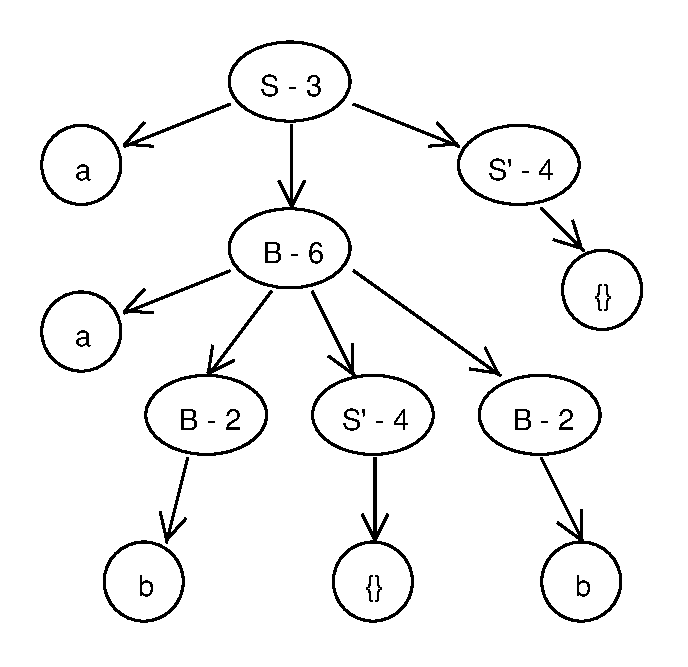
\includegraphics[width=0.4\textwidth,natwidth=458,natheight=444]{umlet/compiled_ex.pdf}
    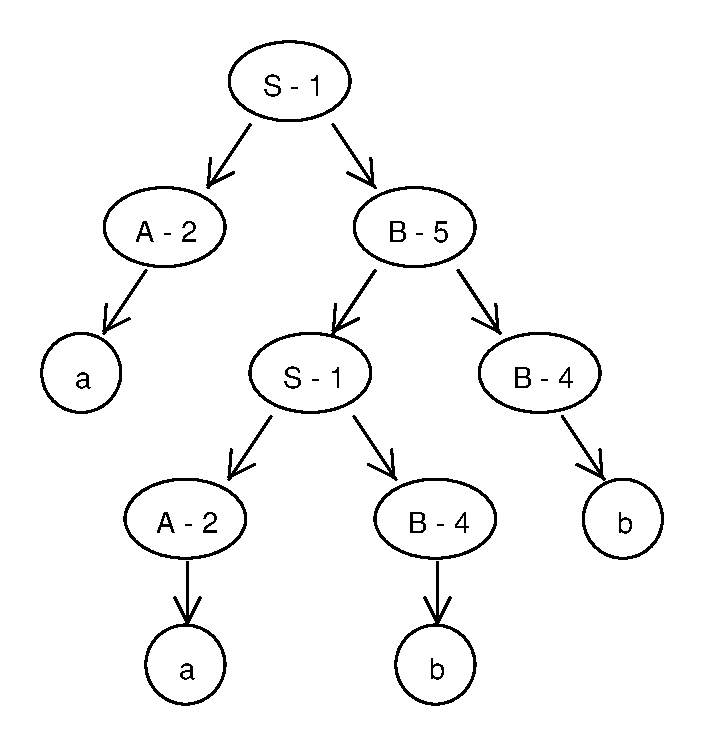
\includegraphics[width=0.4\textwidth,natwidth=472,natheight=500]{umlet/decompiled_ex.pdf}
    \caption{Compiled Grammar Parse Tree (left) Parent Grammar Parse Tree (right)}
    \label{fig:comp_to_dec_ex}
\end{figure}

\clearpage

\section*{Terms}

\begin{itemize}
\item \textbf{Grammar}: a phrase-structure grammar is defined by a finite vocabulary (alphabet), a finite set of
initial strings, and a finite set of rules... \cite{chomsky} (see Production Rule)
\item \textbf{Context-Free Grammar}: a context free grammar is one which only has production rules whose head is a single non-terminal symbol.
\cite{compiler, anatomy, formal_langs}
\item \textbf{Production, Production Rule, Rewrite Rule}: rules of the form $X \rightarrow Y$ where
$X$ and $Y$ are strings in [a grammar]  \cite{chomsky};
define the nonterminal symbols by sequences of terminals and nonterminal symbols \cite{compiler};
rules which specify how nonterminal symbols may be expanded into new sequences of symbols (terminal or otherwise).
\item \textbf{Head (Production Rule)}: the left hand side of a production rule
\item \textbf{Tail (Production Rule)}: the right hand side of a production rule
\item \textbf{Parse Tree}: an ordered, rooted tree whose nodes are symbols in a context-free grammar where the 
children of each brach node correspond to the tail of some production rule in said grammar;
a tree-representation of the grammatical structure of [an input stream] \cite{anatomy}
\item \textbf{Weakly Equivalent (Grammar)}: two grammars are [weakly] equivalent if they define the same language.\cite{reghizzi}
\item \textbf{Strongly/Structurally Equivalent (Grammar)}: two grammars are strongly or structurally equivalent
if they are weakly equivalent and can assign any sentence the same parse tree. \cite{reghizzi}
\end{itemize}

\bibliography{arch}{}
\bibliographystyle{plain}
\end{document}
